\section{User Interface}
The user interface (UI) is perhaps one of the most important aspects of Fidelis; the UI dictates how users interact with the system, and serves as the single point of entry for user data. Fidelis needs to be able to engage the audience from the moment they land on the homepage and encourage the users to explore further by providing an easy to use and intuitive UI. This can be achieved by following standards defined by several committees and adhering to good practices. In addition to the engagement the Fidelis UI must also be usable and simple whilst remaining elegant and intuitive. Responsive design is also crucial to provide access to the system across a range of devices, and this is discussed later in more detail. The provided designs were produced as mock-ups, but were designed in such a way as to closely replicate the final product.

\subsection{Sitemap}
Figure \ref{fig:sitemap} shows the sitemap for Fidelis. This signifies the navigation routes the user will be able to follow on the site. Both sets of users (authorised and authorised) will be able to visit:
\begin{itemize}
\item Discover page - The Discover page will contain posts from a number of categories
\item Profile page - The Profile page will include details on a specific user, including the number of posts they have made and the posts they have voted on
\item Privacy page - The Privacy page will provide details on the Fidelis Privacy policy
\item Support page - The Support page will provide general support to users, such as Frequency Asked Questions (FAQs)
\end{itemize}

However, the Home page, which will contain a feed of posts followed by an authorised user, and the Settings page will only be accessible to authorised users.

\begin{figure}
\centering
\includegraphics[height=2.7in]{Images/Design/sitemap}
\caption{Fidelis Sitemap}
\label{fig:sitemap}
\end{figure}

\subsection{Navigation}
A navigation bar provides users with a quick way of accessing pages on a website. The navigation is usually located at the top of the page, and includes `quick-link' icons that enable the user to easily navigate to pages represented by the icon. Figure \ref{fig:navs} shows the navigation bars for Facebook and Twitter. In both we can see shared elements, such as the profile and home icons. In addition to the icons, the navigation bars also have search boxes. These search boxes enable users to explore content available on each site by providing keywords.

\begin{figure}[H]
\centering
\begin{subfigure}{1\linewidth}
	
\includegraphics[width=1\linewidth]{Images/Design/fb-nav}
	\caption{}
	\label{fig:fb-nav}
\end{subfigure}
\begin{subfigure}{1\linewidth}
	
\includegraphics[width=1\linewidth]{Images/Design/twitter-nav}
	\caption{}
	\label{fig:twitter-nav}
\end{subfigure}
\caption{Navigation bar designs for (a) Facebook and (b) Twitter}
\label{fig:navs}
\end{figure}

By studying existing navigation bar designs, concept designs for navigation on Fidelis were created. These designs can be seen in Figure \ref{fig:fidelis-navs}. There will be two navigation bars - one for unauthorised users and the other for authorised users. Both designs employ intuitive icons that will allow the user to identify the page they will be taken to when the icon is clicked on. To signify the page users are currently on, an orange underline will highlight the icon corresponding to the page the user has navigated to. In addition to this, the navigation bar will also include a search field which will allow the user to locate specific categories or users. The two navigation bars differ slightly in the pages they allow the user to navigate to. When a user is not logged in, they will be unable to view their notifications (signifed by the bell icon), or view their profile. However, they will still be able to view public posts in a category they search for, or view a public user profile.

\begin{figure}[H]
\centering
\begin{subfigure}{1\linewidth}
	
\includegraphics[width=1\linewidth]{Images/Design/nav-unauthorised}
	\caption{}
	\label{fig:nav-unauth}
\end{subfigure}
\begin{subfigure}{1\linewidth}
	
\includegraphics[width=1\linewidth]{Images/Design/nav-authorised}
	\caption{}
	\label{fig:nav-auth}
\end{subfigure}
\caption{Fidelis navigation bar designs for (a) unauthorised and (b) authorised users}
\label{fig:fidelis-navs}
\end{figure}

\subsection{Authentication}
User authentication involves either collecting the credentials of a user to verify their identity and retrieve the relevant data for that user, or allowing a user to register a new account. These two processes for authentication are normally represented with log-in and registration pages. The following sections will look at the design for each of these.

\subsubsection{Log In}
The log-in page should allow an existing user to enter their log-in credentials. On most sites this is a combination of either email or user name, and a password. To be able to correctly verify user identity, both email (or username) and password must be required fields. Users are responsible for remembering the log-in credentials, but are also liable to forget them. To prevent user accounts from being inaccessible, the log-in page should include a link that allows users to recover a forgotten password. A user may accidentally navigate to the log-in page, when they actually intended to navigate to the registration. As such, a link must exist on the log-in page which will take users to the registration page. Figure \ref{fig:login-page} shows the concept design for the log-in page, encapsulated all aforementioned aspects.

\begin{figure}[H]
\centering
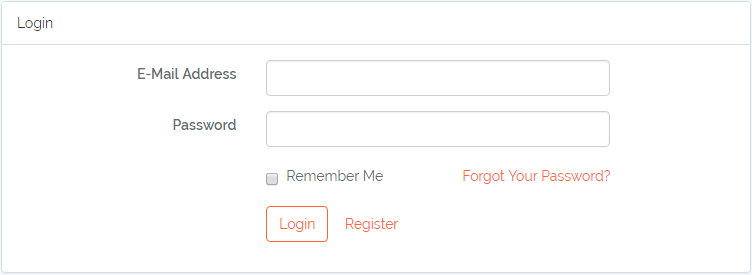
\includegraphics[height=1.5in]{Images/Design/login-page}
\caption{Design for log-in page}
\label{fig:login-page}
\end{figure}

\subsubsection{Register}
The registration page should enable new users to enter their details and create an account on Fidelis. Sites vary in the details they collect during registration. Figure \ref{fig:reg-pages} shows the registration pages for Facebook, Twitter and Reddit. Each of the three sites collects user email addresses and passwords. These two pieces of information are constan across almost all registration pages, regardless of the website. In addition to this, Reddit, as seen in Figure \ref{fig:reddit-reg} asks only for a username. Twitter registration (Figure \ref{fig:twitter-reg}) does not require a username, and instead collect the users full name. Facebook registration collects even more user data, requiring a date of birth and gender in addition to what is already collected by Twitter. 

\begin{figure}
\centering
\begin{subfigure}[b]{.4\linewidth}
	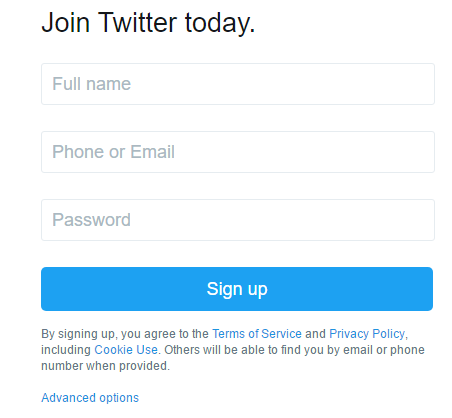
\includegraphics[height=1.5in]{Images/Design/twitter-reg}
	\caption{}
	\label{fig:twitter-reg}
\end{subfigure}
\begin{subfigure}[b]{.5\linewidth}
	\centering
	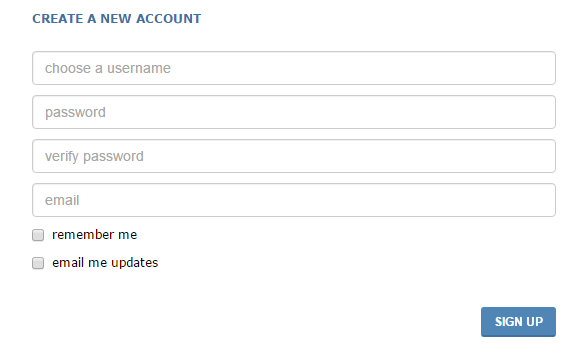
\includegraphics[height=1.5in]{Images/Design/reddit-reg}
	\caption{}
	\label{fig:reddit-reg}
\end{subfigure}
\caption{Registration pages for (a) Twitter and (b) Reddit}
\label{fig:reg-pages}
\end{figure}

Figure \ref{fig:register-page} shows the design for the Fidelis registration page. Users will be required to enter their name, email, username, date of birth and password. Although not entirely necessary initially, it was decided to retain user date of births as thought was put into future uses for it. As the system grows, it is inevitable that certain categories or tags will contain content unsuitable for younger audiences. Therefore, age can be used a tool to filter unsuitable content for younger users.

\begin{figure}[H]
\centering
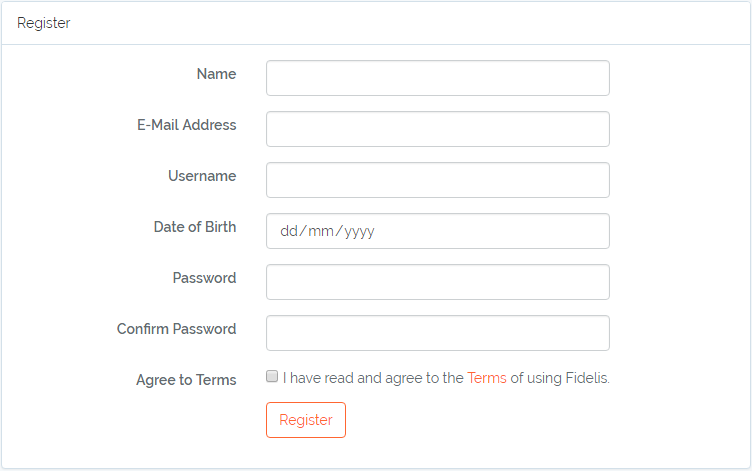
\includegraphics[height=2in]{Images/Design/register-page}
\caption{Design for registration page}
\label{fig:register-page}
\end{figure}

\subsection{Home}
As with most websites, the home page is the central hub from which the user can navigate. This is often the first page that a user will see upon entering the website. Fidelis is no different in this regard. The Fidelis home is split into two different pages, one for when the user is logged in, another for when they aren't.

\subsubsection{Logged Out}
If a user is not logged in to the website, they will see a display shown in Figure \ref{fig:home_unauthorised}. This is the landing page for the site and will be the first port of call for any logged out users or users who are new to Fidelis. The background for this page is a full-screen image, randomly chosen from a select set of images. In the centre of the page there is the title Fidelis, as well as a quote relating to the core concept of the Fidelis platform: trust. Again, these quotes are chosen randomly from a set of quotes. The user can navigate using the buttons in the top right of the page to either log in or sign up for a new account.

\begin{figure}[H]
\centering
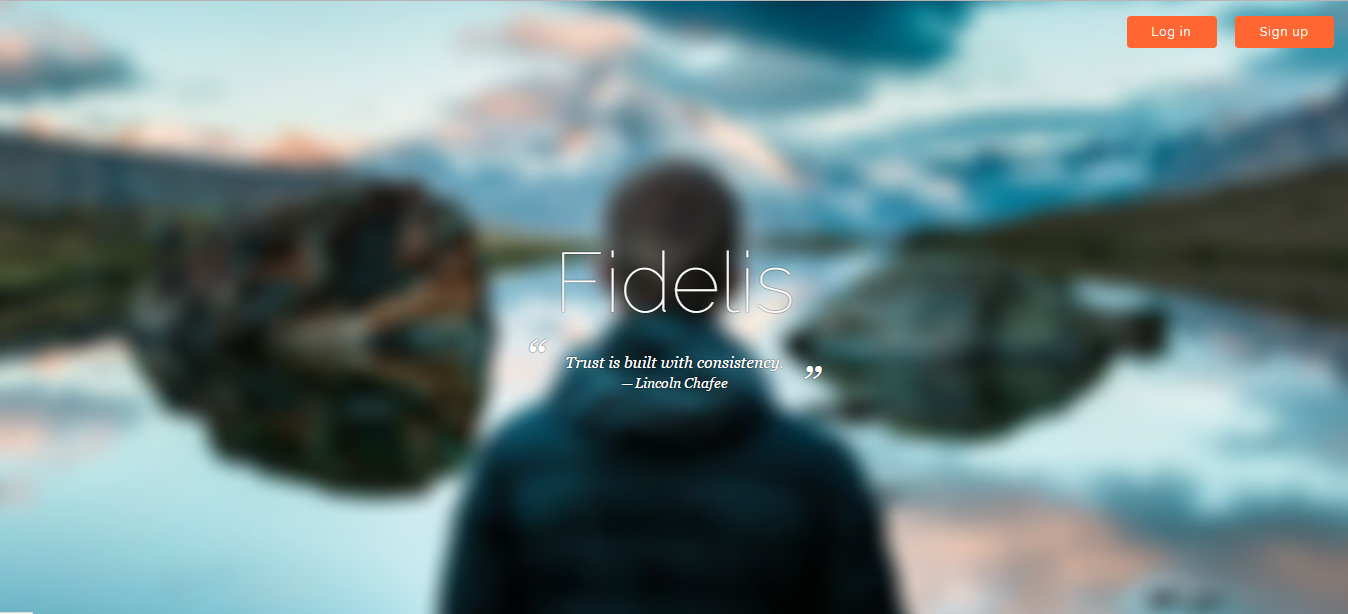
\includegraphics[height=2in]{Images/Design/home_unauthorised}
\caption{Design for Home page when not logged in}
\label{fig:home_unauthorised}
\end{figure}

\subsubsection{Home Page}
Once a user has logged in to their account, the will be directed to the home page, showing in Figure \ref{fig:home_authorised}. The page features the nav bar so the user can navigate to other pages, search for tags/users etc. The most prominent feature of this page is the central post feed. A user can create new posts including text and images as well as interacting with other posts. This includes upvoting or downvoting a post, commenting on a post and reporting posts. The posts displayed in this feed are selected by the system to match the user's interests.

Other than the post feed there are a number of widgets the user can interact with. The user profile widget on the left shows information about the user. This widget links to the user's profile page as well as lists showing the user's posts, the user's followers or other accounts following the user. Also on the left of the page is a widget displaying suggestions for other accounts that the user can follow to expand their network. Again, these suggestions are bespoke for the current user. On the right side of the page is another widget showing the tags that are currently trending across the entire platform. This is another way that the user can find new content rather than seeing just the posts in their feed.

\begin{figure}[H]
\centering
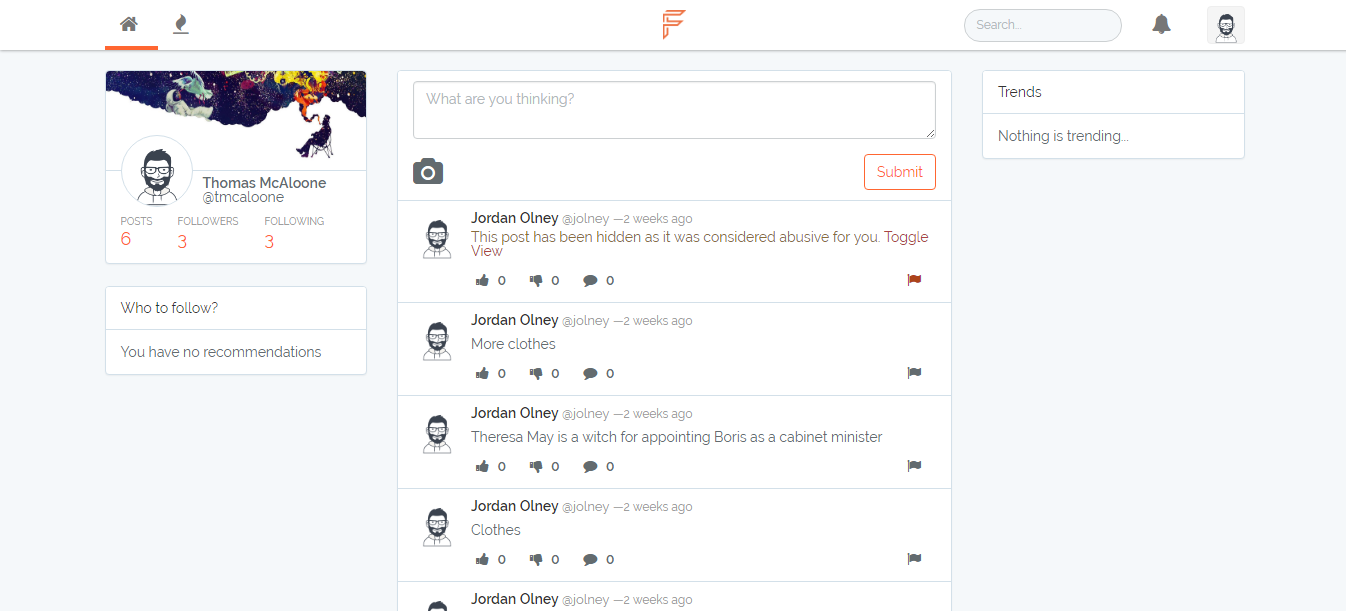
\includegraphics[height=2in]{Images/Design/home_authorised}
\caption{Design for Home page when logged in}
\label{fig:home_authorised}
\end{figure}

\subsection{Discover}

\subsection{Notifications}
Notifications are a key component to communication on social media platforms. Notifications give prompts to users on interactions that have occurred between them and other users. To let users know of a new interactions, notifications either give visual or auditory triggers that get a users attention. With the Google Chrome Notifiations API \cite{ChromeAPI:Notifications} it is now even possible to send notifications to user when they are not on the webpage itself. However, notifications on Fidelis will be provided using a number counter next to a bell icon, which will symbolise the notifications page. This is akin to the notification counter seen on most social media platforms. The page itself will contain a feed of notifications that will give information to the user on who the notification is from, and the type of notification it is. If the notification is a comment, it will include the comment from the user making it. If the notification is for a vote or a follow, it will only include information on the name of the user making the vote or follow. Figure \ref{fig:notifications-page} shows a mock-up of how the notifications page will appear. Hear we can see a number counter next to the bell icon signifying the number of new notifications, and also a notification telling us that another user has commented on one of the posts we have made. In addition to the notifications themselves, the page will also include a profile widget, recommendations widget and trending widget. The user will be able to navigate to their profile from this page, and also interact with trending topics or new user recommendations.

\begin{figure}[H]
\centering
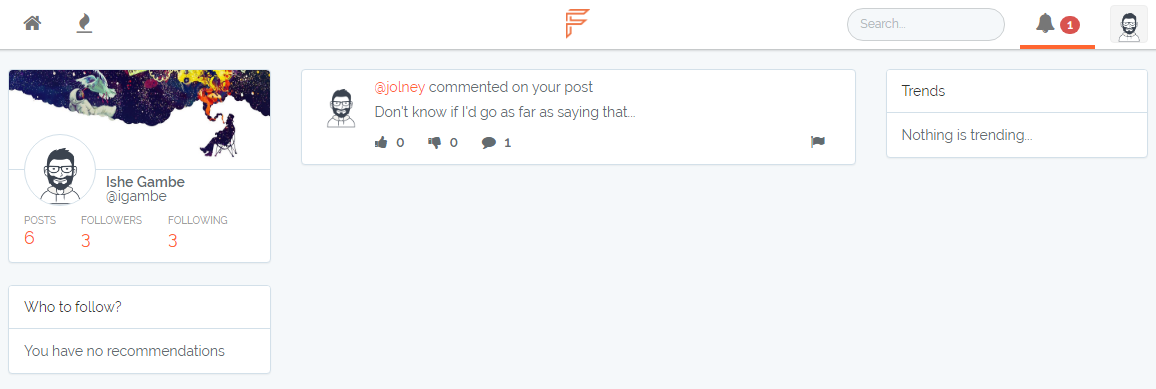
\includegraphics[width=1\linewidth]{Images/Design/notifications-page}
\caption{Design for Notifications page}
\label{fig:notifications-page}
\end{figure}

\subsection{Profile}

\subsection{Settings}

\subsection{Static Pages}

\subsubsection{Privacy Policy}

\subsubsection{Support}